\input{preambulo.tex}

% Titulo
\title[DHCP] {DHCP del Internet Software Consortium}
\author[Carlos Maldonado]{ info@covetel.com.ve \inst{1}}
\subtitle{Fundamentos y Configuraciones Típicas}
\institute[covetel.com.ve]{ \inst{1} Cooperativa Venezolana de Tecnologías Libres R.S. }
\date

\begin{document}

\begin{frame} % (fold)
    \titlepage 
\end{frame}

\begin{frame} % (fold)
    \tableofcontents
\end{frame}

\section{Introducción a DHCP}

\subsection{Fundamentos de DHCP} % (fold)

\label{sub:Fundamentos de DHCP}

% subsection Fundamentos de DHCP (end)

\begin{frame}[allowframebreaks,fragile]{Dynamic Host Control Protocol} % (fold)
    Dynamic Host Control Protocol o \textbf{DHCP} (en castellano, protocolo de
    control de máquinas dinámicas) es el protocolo usado para asignar
    direcciones de manera automática y dinámica en redes de computadores. \\[0.2cm]

    Desarrollado por el Dynamic Host Configuration Working Group del IETF desde
    1993 a 1997 y reflejado en los \textbf{RFC 1351} y \textbf{RFC 2616}. \\[0.2cm]

    El protocolo DHCP esta diseñado para satisfacer la demanda de operaciones
    donde es necesario automatizar la configuración de computadores en red. \\[0.2cm]

    La máquina que efectua la petición se le conoce como \textit{Cliente} y
    existen implementaciones de el programa cliente en practicamente cualquier
    plataforma de hardware y sistema operativo. \\[0.2cm]

    La información transmitida entre cliente y servidor son paquetes no
    superiores a la MTU \textbf{Maximum Transfer Unit} del protocolo de capa 2
    que use la red, tipicamente este protocolo es Ethernet o una de
    sus variantes más rápidas. \\[0.2cm]

    La razón para esta limitación estriba en que es necesario que toda la
    información pueda ser enviada en un solo paquete que será enviado en
    modo broadcast, dado que la máquina cliente que hace la petición, no tiene
    una dirección de red (capa 3) con la cual enviar su paquete y recibir una
    respuesta usando dicha dirección. \\[0.2cm]

    DHCP es un protocolo \textbf{sin estado} (\textit{Stateless}), esto quiere
    decir que no guarda ninguna información sobre conexiones anteriores. La
    única información que se almacena, son las direcciones que se han entregado
    (arrendado) a los distintos clientes que han hecho peticiones.\\[0.2cm]

    Además de la dirección IP, existen otros valores de configuración que se
    pueden establecer mediante el uso de DHCP. Routers por omisión, DNS
    primario y secundario, máscara de red, dirección de broadcast y servidores
    WINS, entre otras.\\[0.2cm]

\end{frame} 

\begin{frame}[allowframebreaks,fragile]{Mitos comunes detrás del DHCP} % (fold)

    \textbf{Exceso de tráfico broadcast:} es un mal concepto ampliamente
    difundido, que DHCP generaría una gran cantidad de tráfico \textit{broadcast},
    en realidad la cantidad de \textit{broadcast} es mínima. En el peor de los
    casos, con un cliente de capacidades limitadas, el intercambio de paquetes
    broadcast serían cuatro.\\[0.2cm]
    
    En el mejor de los casos, que comprende una gran mayoría de los sistemas
    operativos, el cliente necesitaría solo enviar un paquete \textit{broadcast}
    y no requeriría una respuesta \textit{broadcast}. La mayoría de los servidores
    también pueden responder en modo \textit{unicast}.\\[0.2cm]

    Otro mito es que el \textit{broadcast} abarcaría toda red corporativa,
    cuando en realidad, solo esta limitado al segmento de red donde la máquina
    cliente del DHCP está conectada. El resto del tráfico sería \textit{unicast}.\\[2cm]

    \textbf{Exceso de carga en el servidor:} otro concepto común es que un
    servidor DHCP necesitaría mucho poder de cómputo para brindarle servicio a
    miles de máquinas. Sin embargo, es posible darle servicio a alrededor de
    10.000 clientes con una máquina 486 con Linux.\\[0.2cm]

\end{frame} 

\subsection{Asignación de direcciones} % (fold)


\begin{frame}[allowframebreaks,fragile]{Tipos de asignación} % (fold)
    \textbf{Asignación estática:} el servidor recibe una listado con
    información que identifica a los clientes DHCP. Dicho listado permite
    diferenciar a cada uno de los clientes. Para cada identificador, se
    establece una dirección IP que debe ser asignada a dicho cliente.
    Si el cliente es móvil, debe haber una direccción para dicho
    dispositivo en cada rango de la red. \\[0.2cm]

    \textbf{Asignación dinámica:} el servidor recibe un rango de direcciones
    para cada segmento de red donde se espera que hayan clientes DHCP. Cuando
    el cliente solicita una dirección, el servidor consigue una dirección
    disponible en dicho segmento de red para entregarla al cliente.\\[0.2cm]

    \textbf{Asignación automática:} el servidor asigna una dirección de la
    misma manera que en el método dinámico, solo que dicha dirección se asigna
    de manera permanente al mismo cliente. Una manera aproximada de usar dicho
    modo de asignación es utilizar \textit{leases} muy largos.\\[0.2cm]

    \framebreak

    \textbf{Asignación híbrida:} existen una variedad de métodos híbridos que
    son posibles con DHCP. Por ejemplo una estrategia común es asignar
    direcciones fijas a los clientes DHCP registrados, permitiendo que los
    clients DHCP no registrados adquieran direcciones IP asignadas de manera
    dinámica.\\[0.2cm]

    Cual de estas estrategias ha de utilizarse en una red en particular, es una
    decision que queda de parte del administrador. Obviamente, mantener un
    registro de todos los clientes DHCP conectados en una red es una carga de
    trabajo considerable que en algunos entornos vale la pena.\\[0.2cm]

    Es necesario resaltar que DHCP no debe usarse como mecanismo de seguridad,
    si el cliente DHCP elige no seguir el protocolo, el administrador puede
    hacer poco más que, detectar el dispositivo y bloquearlo. Usar control de acceso
    puede ser conveniente, pero no evita el acceso no autorizado a una
    red.\\[0.2cm]
    
\end{frame}

\subsection{Funciones principales del DHCP} % (fold)
\label{sub:Funciones principales del DHCP}

% subsection Funciones principales del DHCP (end)

\begin{frame}{Arrendado (leasing)} % (fold)

    Tal y como se explicó que el servidor DHCP es \textit{Stateless} y
    opera de manera automática, este no puede saber que ha pasado con los
    dispositivos después de que se les asigna una dirección. En vez de asignar una
    dirección IP a cada cliente hasta que este termine de usarla, el servidor
    DHCP asigna una dirección con un \textit{lease} y el cliente esta
    autorizado a usarla hasta el final de la duración de dicho
    \textit{lease}.\\[0.2cm]


\end{frame}

\begin{frame}{Reclamación (reclamation)} % (fold)

    Al restringir los clientes a usar direcciones IP, solo hasta que expiren
    los \textit{leases} y al proveer un mecanismo para que actualicen los
    \textit{leases} mientras esten activos y conectados a la red, DHCP permite
    'reclamar' las direcciones IP que no están en uso. Si un dispositivo esta
    apagado por un periodo extendido de tiempo, debe contactar al servidor DHCP
    y solicitar una dirección cuando se activa. Si la dirección anterior no
    está disponible, se le ofrece una nueva dirección. Esto evita la mayoría de
    los conflictos de asignación de direcciones.

\end{frame}

\begin{frame}{Liberación (release)} % (fold)

    Un cliente puede renunciar a su \textit{lease} sobre una dirección, antes
    de su expiración, por ejemplo cuando una máquina va a moverse de una red a
    otra, de manera que el servidor sepa que la dirección queda disponible
    inmediatamente para ser reasignada. Algunos clientes DHCP pueden
    configurarse para renunciar a su dirección cada vez que la máquina se
    apaga. El cliente no espera una respuesta a dicha transacción.

\end{frame}

\begin{frame}{Descripción de servicios} % (fold)

   Además de distribuir direcciones IP, DHCP permite configurar información que
   sea distribuida en la forma de opciones de DHCP, incluyendo las siguientes:

   \begin{itemize}
       \item Dirección del router por omisión
       \item Dirección(es) de servidor(es) DNS
       \item Nombre del archivo para hacer boot de una máquina (para dispositivos que inician
       cargando archivos desde un dispositivo de almacenamiento disponible en
       la red)
       \item Nombre del sistema de archivos y servidor de swap (para clientes
       DHCP sin disco)
   \end{itemize}

\end{frame}

\subsection{Ejemplo inicial de funcionamiento} % (fold)
\label{sub:Ejemplo inicial de funcionamiento}

% subsection Ejemplo inicial de funcionamiento (end)

\begin{frame}[allowframebreaks,fragile]{Ejemplo básico de direccionamiento DHCP} % (fold)

    A continuación veremos una red de ejemplo en la organización ficticia MAY,
    cinco segmentos de red, todos ellos conectados entre si por un router que
    a su vez los conecta a Internet. Cuatro segmentos de red son usados por las
    estaciones de escritorio del personal de la empresa, el segmento restante
    se usa para los servidores que se encuentran alojados en el centro de
    datos. 

    \begin{figure}
    \begin{center}

    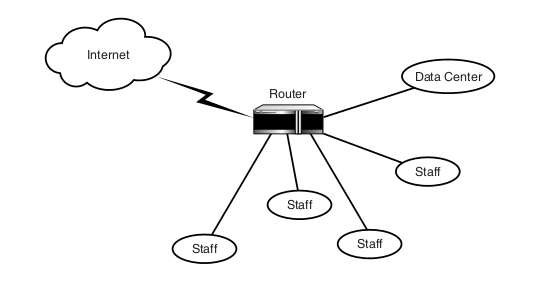
\includegraphics[scale=0.65]{images/2-1.png}
    \caption{Diagrama de la red MAY}
    \label{MAY-1}

    \end{center}
    \end{figure}

    El administrador de la red, ha obtenido cinco redes IP clase C desde la
    192.168.11.0 hasta la 192.168.15.0 y se han asignado a los segmentos de red
    como se muestran en la siguiente figura 

    \begin{figure}
    \begin{center}

    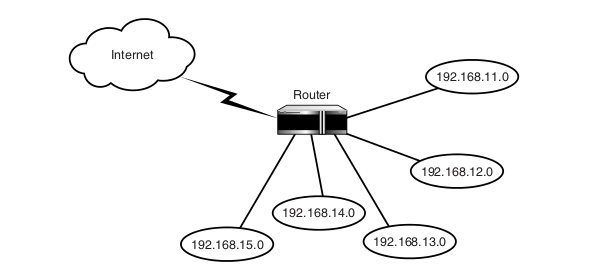
\includegraphics[scale=0.65]{images/2-2.png}
    \caption{Diagrama de la red MAY con direcciones de red}
    \label{MAY-2}

    \end{center}
    \end{figure}

    El objetivo es lograr que un servidor DHCP se encargue de gestionar la
    configuración de las computadoras conectadas a la red MAY. Ahora
    describiremos brevemente las interacciones entre un computador de
    escritorio y el servidor DHCP de la red MAY, en las siguientes instancias:

    \begin{itemize}
        \item Cuando un computador se conecta por primera vez a la red MAY
        \item Cuando un computador se reinicia
        \item Cuando un computador es cambiado de ubicación dentro de la red MAY
        \item Cuando un computador es eliminado de la red MAY
    \end{itemize}

    \begin{figure}
    \begin{center}

    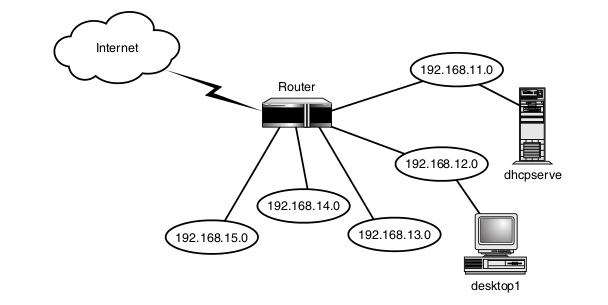
\includegraphics[scale=0.65]{images/2-3.png}
    \caption{Diagrama de la red MAY - Cliente - Servidor }
    \label{MAY-3}

    \end{center}
    \end{figure}

\end{frame}

\begin{frame}[allowframebreaks,fragile]{Cuando un computador se conecta por primera vez a la red
MAY} % (fold)

    Cuando \textit{desktop1} se conecta por primera vez a la red MAY, necesita
    contactar al servidor DHCP para obtener una dirección IP y otros parámetros
    de configuración. Para ubicar un servidor DHCP, \textit{desktop1} envía un
    mensaje broadcast \textit{desktop1} para ubicar potenciales servidores
    DHCP en la red MAY.\\[0.2cm]

    Luego \textit{dhcpserve} recibe este \textit{broadcast} y responde a
    \textit{desktop1} identificándose como un servidor DHCP. Como
    \textit{desktop1} y \textit{dhcpserve} están en distintos segmentos de red,
    el router actuando como \textit{relay agent}, reenvia los mensajes entre
    ambos computadores. En diapositivas posteriores, se explicará esto con
    detalle.\\[0.2cm]

    Después de \textit{dhcpserve} recibir el mensaje inicial de
    \textit{desktop1}, \textit{dhcpserve} selecciona una dirección IP que es
    adecuada para la red 192.168.12.0 a la que \textit{desktop1} está
    conectada. Además otros parámetros de configuración son enviados, como por
    ejemplo: la máscara de red, la dirección de la interfaz de red del router
    en la red 192.168.12.0 y la dirección del servidor DNS en la red
    MAY.\\[0.2cm]

\end{frame}


\begin{frame}[fragile]{Cuando un computador se reinicia} 

    Lorem Ipsum

\end{frame}


\begin{frame}[fragile]{Cuando un computador cambia de sitio dentro de
la red MAY} 

    Lorem Ipsum

\end{frame}


\begin{frame}[fragile]{Cuando un computador es eliminado de la red MAY}

    Lorem Ipsum

\end{frame}

\end{document}
